\section{The original character lift and its complete supported
return}\label{the-original-character-lift-and-its-complete-supported-return}

\begin{figure}
\centering
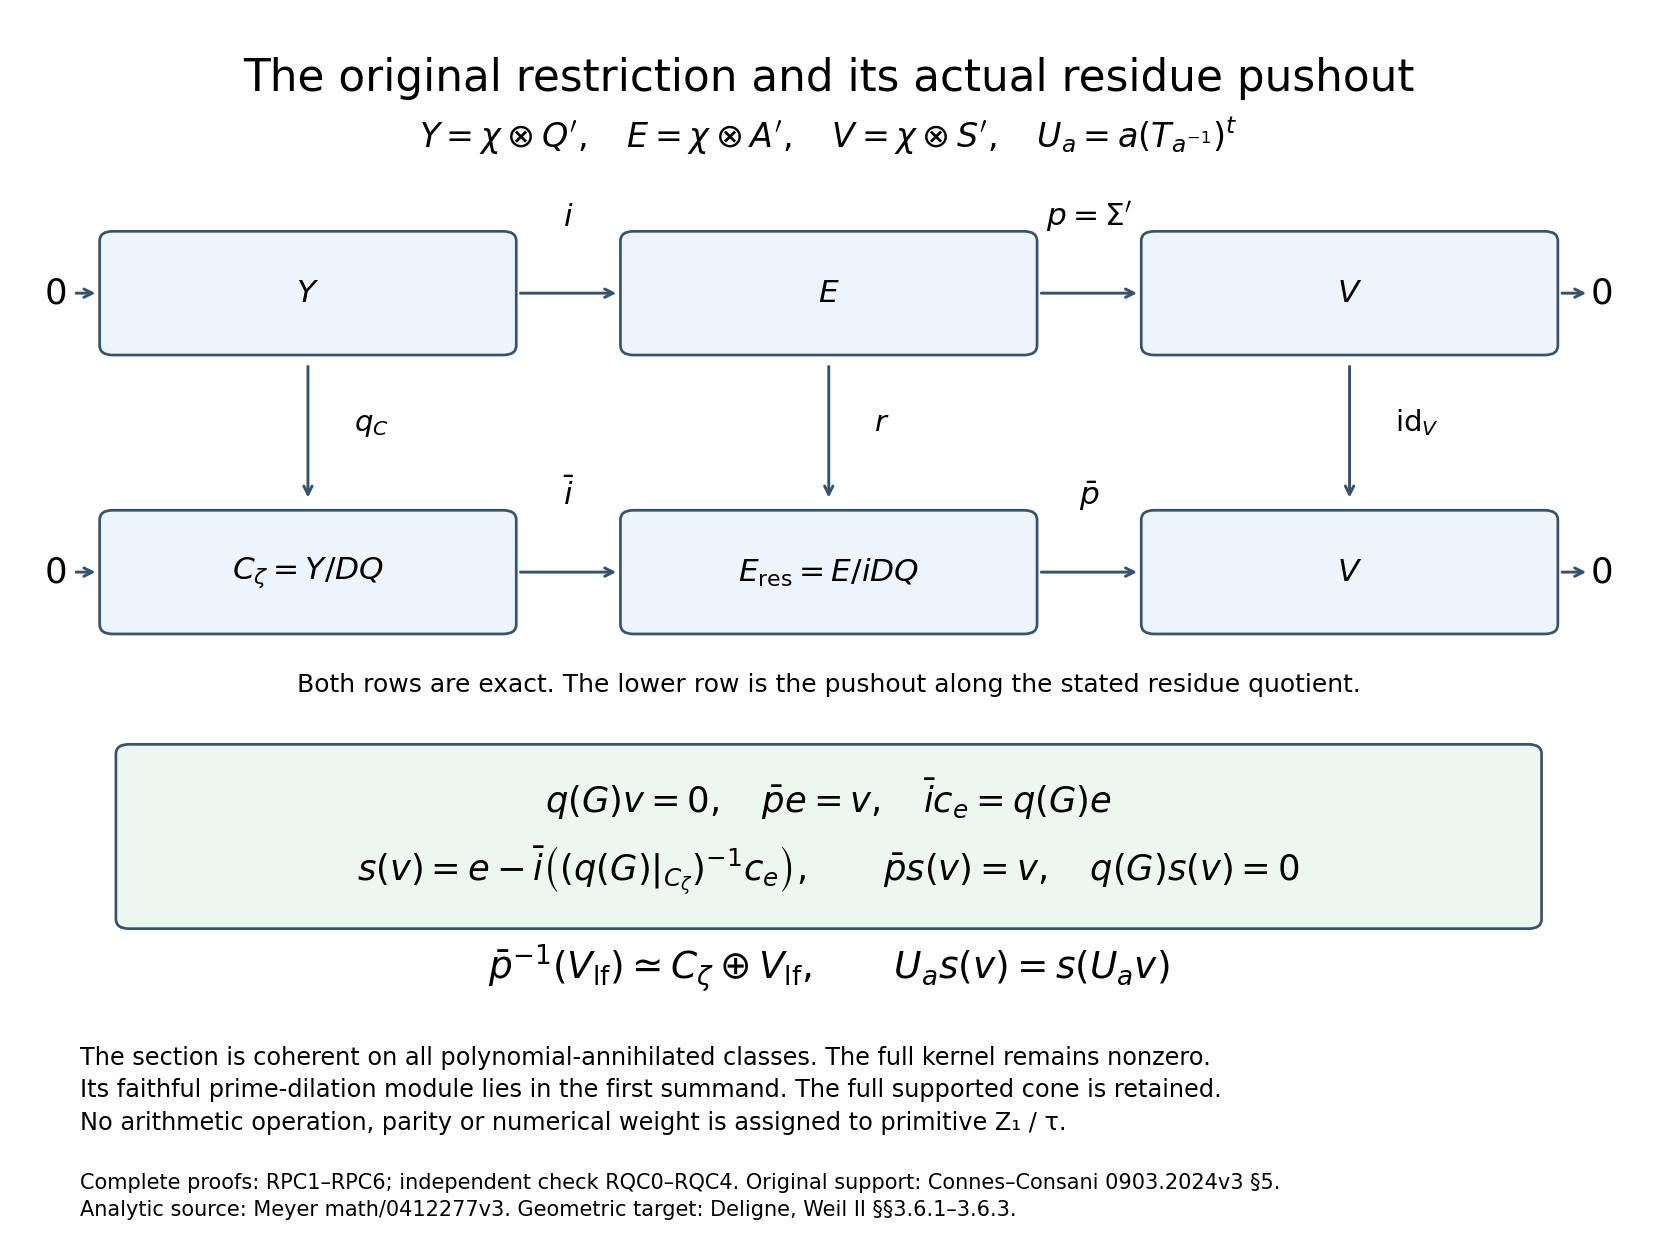
\includegraphics[width=\textwidth,height=.83\textheight,keepaspectratio]{tau_lifting_weights_20260924/ACTUAL_RESIDUE_PUSHOUT.png}
\caption{The original restriction and its actual residue pushout}
\end{figure}

Figure 1. Both exact rows, the actual pushout, its cochain placement and
the coherent full-group-equivariant section are proved in
\href{ACTUAL_RESIDUE_PUSHOUT_AND_CHARACTER_LIFTING.md}{RPC1--RPC5},
independently checked in
\href{ACTUAL_RESIDUE_PUSHOUT_INDEPENDENT_CHECK.md}{RQC0--RQC3}. Every
polynomial inverse is the earlier constructed operator on the actual
C\_zeta. The full prime-dilation kernel remains. The source Z\_0,
primitive Z\_1/tau and integer Z\_2 keep their original definitions and
retractions; the diagram operates on the constructed receiving spaces.

\begin{figure}
\centering
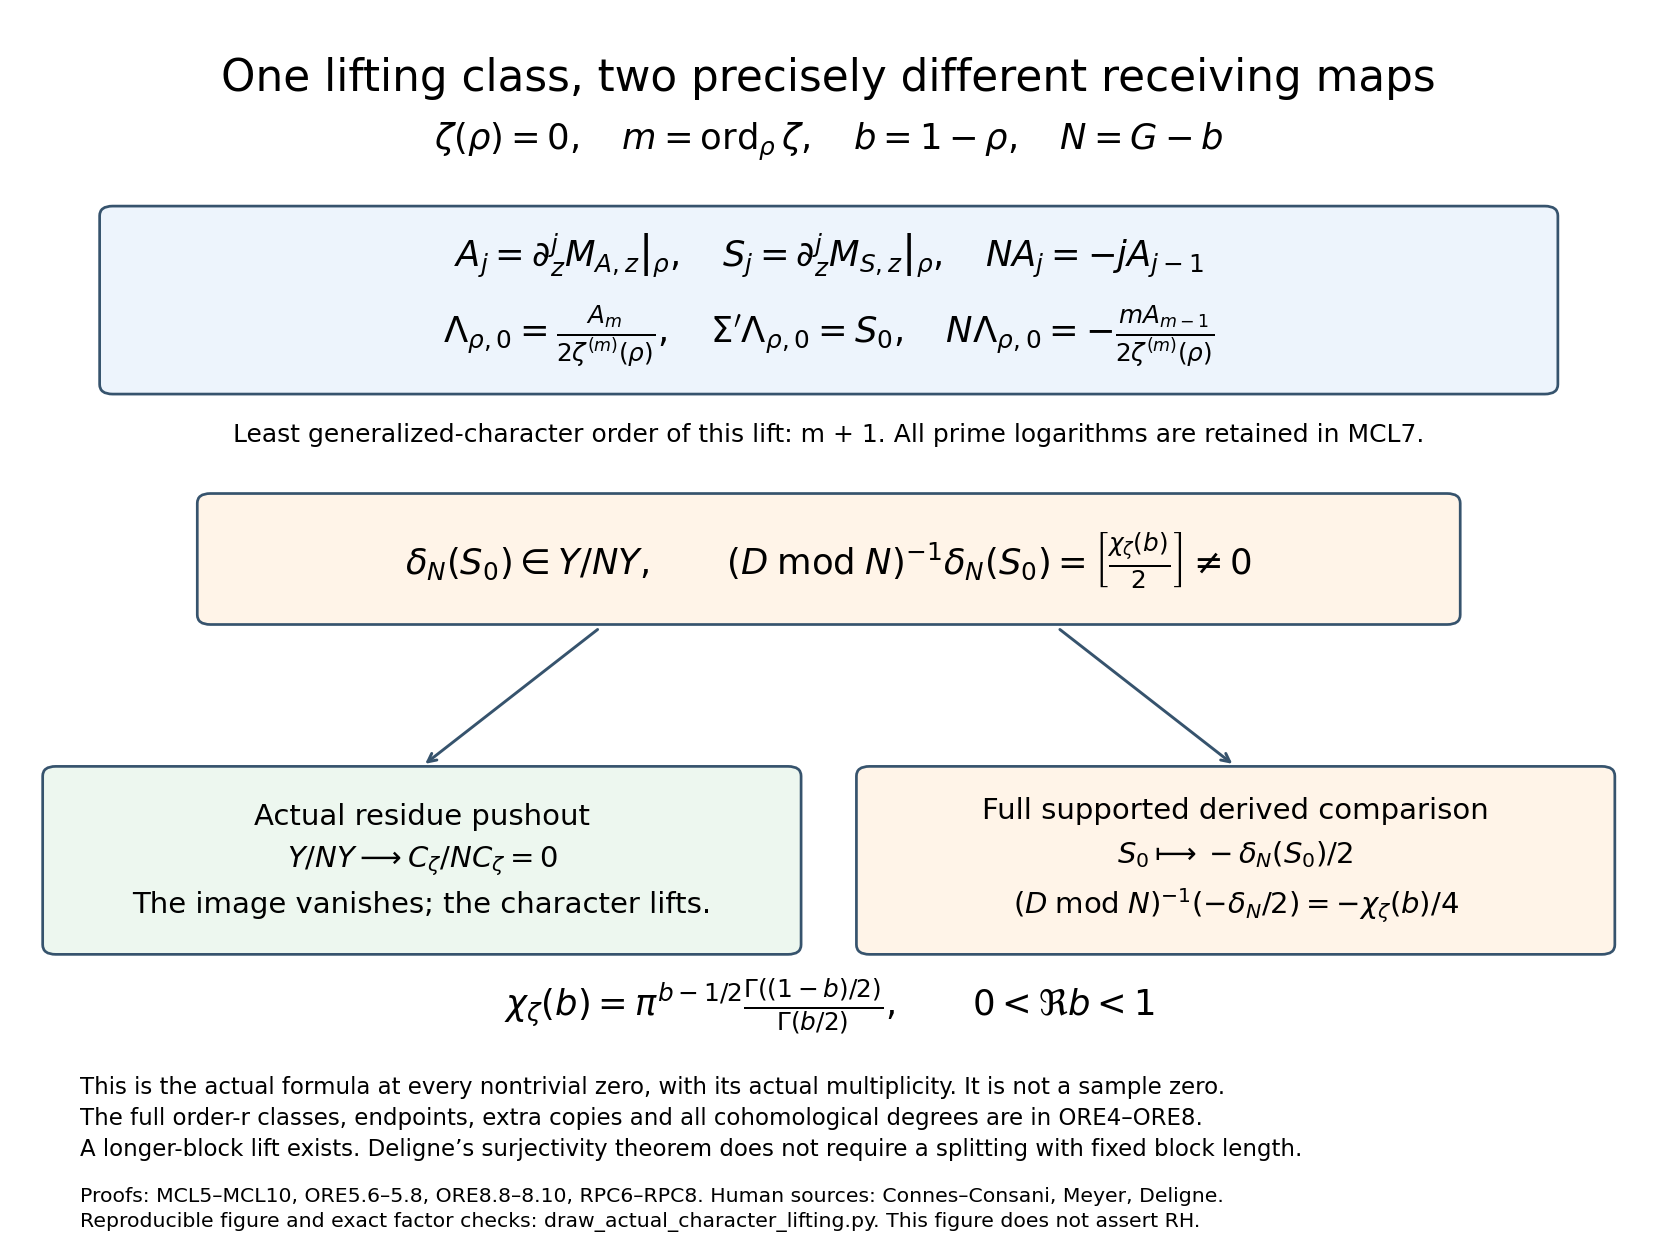
\includegraphics[width=\textwidth,height=.83\textheight,keepaspectratio]{tau_lifting_weights_20260924/ACTUAL_SUPPORTED_CHARACTER_CLASS.png}
\caption{One exact extension class under two different receiving maps}
\end{figure}

Figure 2. This is an exact formula at every actual nontrivial zero, with
its actual multiplicity m, not a numerical example or an assumed
multiple zero. \href{ORIGINAL_MELLIN_CHARACTER_LIFTING.md}{MCL5--MCL10}
proves the least lift order and every real/prime action.
\href{ORIGINAL_RESTRICTION_EXTENSION_AND_DELIGNE_CROSS.md}{ORE5.6--ORE5.8
and ORE8.8--ORE8.10} proves the full higher-jet class and its actual
supported return.
\href{ACTUAL_RESIDUE_PUSHOUT_AND_CHARACTER_LIFTING.md}{RPC6--RPC8} gives
both exact receiving maps. The complete Gamma multiplier, raw derivative
coefficients and signs remain in those formulas. All other cohomological
degrees, four endpoint lines, and both complete extra closed copies
remain in ORE8.7.

Reproducible vector/raster source: draw\_actual\_character\_lifting.py.
Both final PNGs were inspected. Its 105 exact rational checks verify
finite instances of the general lift, generator, connecting-rank and
residue-transport formulas; they supplement the complete proofs and are
not numerical tests of RH.

Human sources: Alain Connes and Caterina Consani,
\href{https://arxiv.org/abs/0903.2024v3}{0903.2024v3 §5}; Ralf Meyer,
\href{https://arxiv.org/abs/math/0412277v3}{math/0412277v3, The spectral
interpretation}; Pierre Deligne,
\href{https://www.numdam.org/item/PMIHES_1980__52__137_0/}{Weil II
§§3.6.1--3.6.3}. Author-source identities and the explicitly identified
French transcription of Deligne are recorded with exact reading coverage
in the source ledger. No geometric weight-separation or RH conclusion is
supplied by these diagrams.
